%----------------------------------------------------------------------------------------
%	Modified class referred tex document.
%----------------------------------------------------------------------------------------

\documentclass[]{CKAgn}
\ckasetup{ 
  type={Example},
  author={Yuchen Jin},
  organization={Test the organization},
  number={1},
  textStyle={box}
}
\usepackage{metalogo}
\usepackage{lipsum}

\begin{document}

\maketitle % Print the title

\CKAcontents[2col]{}

\section{Introduction}

In this example, we show the basic functions of this class. This class is both compatible with pdf\LaTeX and \XeLaTeX.

\lipsum[2-3]

\section{Example environments}

\subsection{Example of figure}
Here we show \autoref{fig:res:a} and \autoref{fig:res:b}.
\begin{figure}[htbp] \label{fig:res}
  \centering
  \subfloat[test1]{ \label{fig:res:a}
    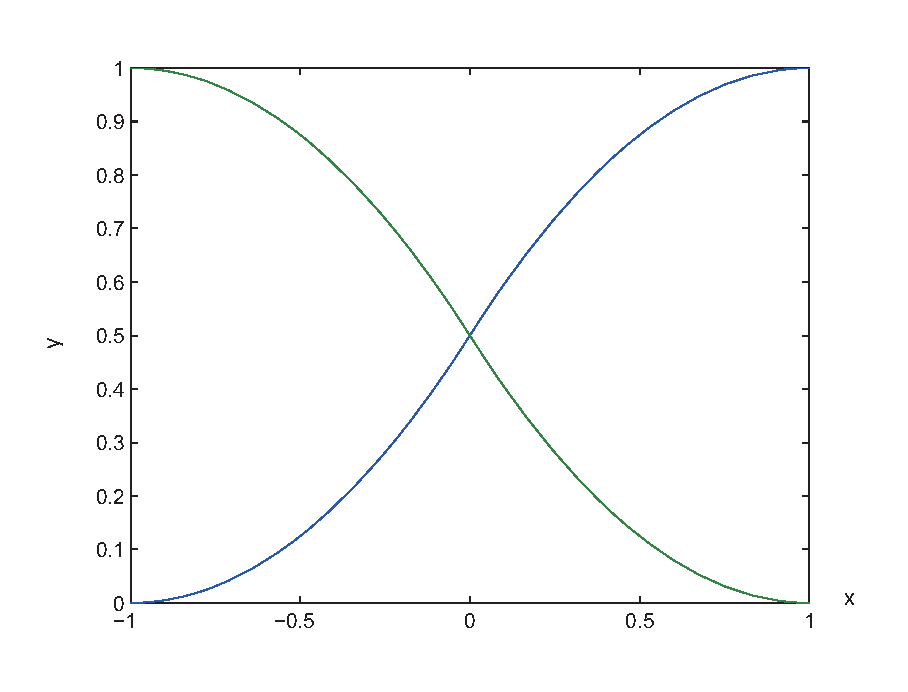
\includegraphics[width = 0.4\columnwidth]{test1}
  }
  \subfloat[test2]{\label{fig:res:b}
    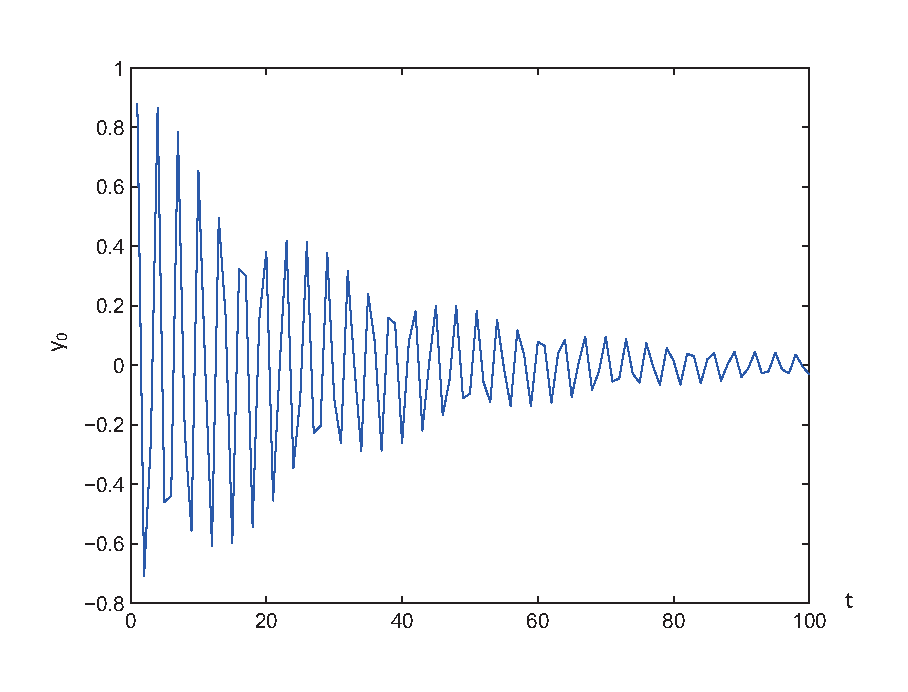
\includegraphics[width = 0.4\columnwidth]{test2}
  }
  \DeclareGraphicsExtensions.
  \caption{Test graphs.}
\end{figure}

\subsection{Example of table}

Here we show an example, \autoref{tab:Table1}.

\begin{table}[htbp]
  \centering
  \caption{Example table \label{tab:Table1}}
  \begin{tabular}{|m{0.1\columnwidth}<{\centering}|m{0.46\columnwidth}|}
    \hline
    \textbf{Symbol} & \makebox[0.46\columnwidth][c]{\textbf{Description}} \\ \hline
    $\alpha$ & text 1 \\ \hline
    $\Gamma$ & text 2 \\ \hline
    $\Omega$ & text 3 \\ \hline
  \end{tabular}
\end{table}

Here we show another table, \autoref{tab:Table2} is long and breakable.

\begin{longtable}{|m{0.1\columnwidth}<{\centering}|m{0.46\columnwidth}|}
  \caption{Example long table\label{tab:Table2}} \\
  \hline
  \textbf{Symbol} & \makebox[0.46\columnwidth][c]{\textbf{Description}} \\ \hline
  $\alpha$ & text 1 \\ \hline
  $\Gamma$ & text 2 \\ \hline
  $\Omega$ & text 3 \\ \hline
  $\chi$ & a lot of rows \\ \hline
  $\chi$ & a lot of rows \\ \hline
  $\chi$ & a lot of rows \\ \hline
  $\chi$ & a lot of rows \\ \hline
  $\chi$ & a lot of rows \\ \hline
  $\chi$ & a lot of rows \\ \hline
\end{longtable}

\subsection{Example of theorem}

We refer \autoref{thm:theorem1} and \autoref{que:question1} respectively.

\begin{theorem}[Title] \label{thm:theorem1}
  Here we show an theorem.
\end{theorem}

\begin{question}[Special exercise] \label{que:question1}
  Here we show a question.
\end{question}

\subsection{Example of algorithm}

Test Algorithm in \autoref{alg::Algorithm}:

\begin{algorithm}[!htbp]
  \caption{DWT Algorithm}
  \label{alg::Algorithm}
  \begin{algorithmic}[1]
    \REQUIRE Sequence $\mathbf{x}$ in time domain
    \ENSURE Sequence $\hat{\mathbf{x}}$ in wavelet domain
    % if-then-else
    \STATE N = $\left\lfloor \log_2 (\mathrm{length}(\mathbf{x})) \right\rfloor$;
    \STATE $\mathbf{c}_{N} = \mathbf{x},~ \hat{\mathbf{x}} = \varnothing$;
    \FOR{$i$ from $1$ to $N$}
    \STATE $\mathbf{c}_{N-i},~\mathbf{d}_{N-i}~=~\mathrm{analysis\_filter}(\mathbf{c}_{N-i+1})$;
    \STATE insert $\mathbf{d}_{N-i}$ at the beginning of $\hat{\mathbf{x}}$.
    \ENDFOR
  \end{algorithmic}
\end{algorithm}

\section{Example of special text}

My name is \change{Yuccn}{Yuchen} Jin, I am a graduate \err{school} student of University of Houston. My major is Electrical \add{and Computer} Engineering. I am not certain about whether \unsure{I am a top student}. Now I believe that I should not discuss about \change{this topic}{the topic about myself}.

\end{document} 